% -*- TeX:de -*-
\NeedsTeXFormat{LaTeX2e}
\documentclass[12pt,a4paper]{article}
\usepackage[german]{babel} % german text
\usepackage[DIV12]{typearea} % size of printable area
\usepackage[T1]{fontenc} % font encoding
%\usepackage[latin1]{inputenc} % most likely on Windows
\usepackage[utf8]{inputenc} % probably on Linux
\usepackage{multicol}

% PLOTTING
\usepackage{pgfplots} 
\usepackage{pgfplotstable}
\usepackage{url}
\usepackage{graphicx} % to include images
\usepackage{tikz}
\usepackage{subfigure} % for creating subfigures
\usepackage{amsmath} % a bunch of symbols
\usepackage{amssymb} % even more symbols
\usepackage{booktabs} % pretty tables
\usepackage{makecell} % multi row table heading

% a floating environment for circuits
\usepackage{float}
\usepackage{caption}

%\newfloat{circuit}{tbph}{circuits}
%\floatname{circuit}{Schaltplan}

% a floating environment for diagrams
%\newfloat{diagram}{tbph}{diagrams}
%\floatname{diagram}{Diagramm}

\selectlanguage{german} % use german

\begin{document}








%%%% TO DO
%
% - - Shorty:
%

% - - Patrick
%




%%%%%%% DECKBLATT %%%%%%%
\thispagestyle{empty}
			\begin{center}
			\Large{Fakultät für Physik}\\
			\end{center}
\begin{verbatim}


\end{verbatim}
							%Eintrag des Wintersemesters
			\begin{center}
			\textbf{\LARGE WS 2013/14}
			\end{center}
\begin{verbatim}


\end{verbatim}
			\begin{center}
			\textbf{\LARGE{Physikalisches Praktikum\\ für das Bachelorstudium}}
			\end{center}
\begin{verbatim}




\end{verbatim}

			\begin{center}
			\textbf{\LARGE{PROTOKOLL}}
			\end{center}
			
\begin{verbatim}





\end{verbatim}

			\begin{flushleft}
			\textbf{\Large{Experiment (Nr., Titel):}}\\
							%Experiment Nr. und Titel statt den Punkten eintragen
			\LARGE{PW5 Gasthermometer, Adiabatenkoeffizienten, Dampfdichte}	
			\end{flushleft}

\begin{verbatim}

\end{verbatim}	
							%Eintragen des Abgabedatums, oder des Erstelldatums des Protokolls
			\begin{flushleft}
			\textbf{\Large{Datum:}} \Large{07.11.2013}
			\end{flushleft}
			
\begin{verbatim}
\end{verbatim}
							%Namen der Protokollschreiber
		\begin{flushleft}
			\textbf{\Large{Namen:}} \Large{Patrick Braun, Johannes Kurz}
			\end{flushleft}

\begin{verbatim}


\end{verbatim}
							%Kurstag und Gruppennummer, zb. Fr/5
			\begin{flushleft}
			\textbf{\Large{Kurstag/Gruppe:}} \Large{DO/2}
			\end{flushleft}

\begin{verbatim}



\end{verbatim}
							%Name des Betreuers, das Praktikum betreute.
			\begin{flushleft}
			\LARGE{\textbf{Betreuer:}}	\Large{ Franz Sachslehner }	
			\end{flushleft}

%%%%%%% DECKBLATT ENDE %%%%%%%
\pagebreak
\setlength{\columnsep}{20pt}
\begin{multicols}{2}

%%%%%%%%%%%%%%%%%%%%%%%%%%%%%%%%%%%%
\section{Gasthermometer}
Im ersten Teil von PW5 sollen das Boyle-Mariotte'sche Gesetz für ideale Gase und deren Spannungskoeffizient $\beta$ bestimmt werden.\\
Ein idealisiertes Gas hat einen einfachen Zusammenhang zwischen Volumen, Druck und Temperatur und ist dadurch gekennzeichnet, dass Interaktion zwischen seinen Molekülen und deren Volumen vernachlässigbar sind.\\
In diesem Versuch ist Luft das Gas, dessen Volumen und Druck betrachtet werden. Bei Raumtemperatur ist Luft weit vom Phasenübergang zur Flüssigkeit entfernt und kann daher näherungsweise als ideales Gas betrachtet werden.\\
Eine Eigenschaft wird durch das Boyle-Mariotte'sche Gesetz beschrieben:\\
$p\cdot V= const$
Also bei konstanter Temperatur ist auch das Produkt aus Druck und Temperatur (für alle Kombinationen) konstant.\\
Zum Nachweis wird ein \textbf{Gasthermometer} verwendet: 2 Glasgefäße sind über einen Schlauch miteinander verbunden und parallel an einer Messskala angebracht. In dem System befindet sich Quecksilber. Das eine Gefäß ist abgeschlossen und enthält eine Luftkammer, abgeschlossen vom Quecksilber (Messgefäß). Das andere Gefäß ist offen, sodass der Umgebungsluftdruck auf das Quecksilber wirkt (siehe Abbildung \ref{fig:gas_therm_aufbau}).\\
Verschiebt man die beiden Behälter zueinander, lassen sich, bei konstanter Temperatur, verschiedene Luftvolumina im Messgerät sowie Höhendifferenzen der beiden Quecksilbersäulen ablesen.\\
Die Quecksilber-Höhendifferenz addiert (oder subtrahiert) zum Außenluftdruck ergibt den Druck, der in der Luftkammer herrscht. Die Produkte der Volumen/Druck-Paare sollen für alle Kombinationen gleich sein.\\
\\
Außerdem soll der Spannungskoeffizient $\beta$ von Luft bestimmt werden. Dieser sollte $\frac{1}{T_0}$ sein, wobei $T_0 = 273.15K$. Dieser ist der Faktor, mit dem sich der Druck eines idealen Gases bei konstant gehaltenem Volumen linear mit der Temperatur ändert.\\
Das Volumen der Luftkammer des Gasthermometers wird konstant gehalten, während der Druck bei verschiedenen Temperaturen bestimmt wird. Aus 
$$ \beta = \frac{1}{p_0} \cdot \frac{\Delta p}{\Delta \vartheta} $$
lässt sich der Spannungskoeffizient durch einen linearen Fit der Druck/Temperatur-Wertepaare bestimmen ($p_0$ ist dabei der Druck bei $T_0$.

\begin{figure}[H]
	\centering
	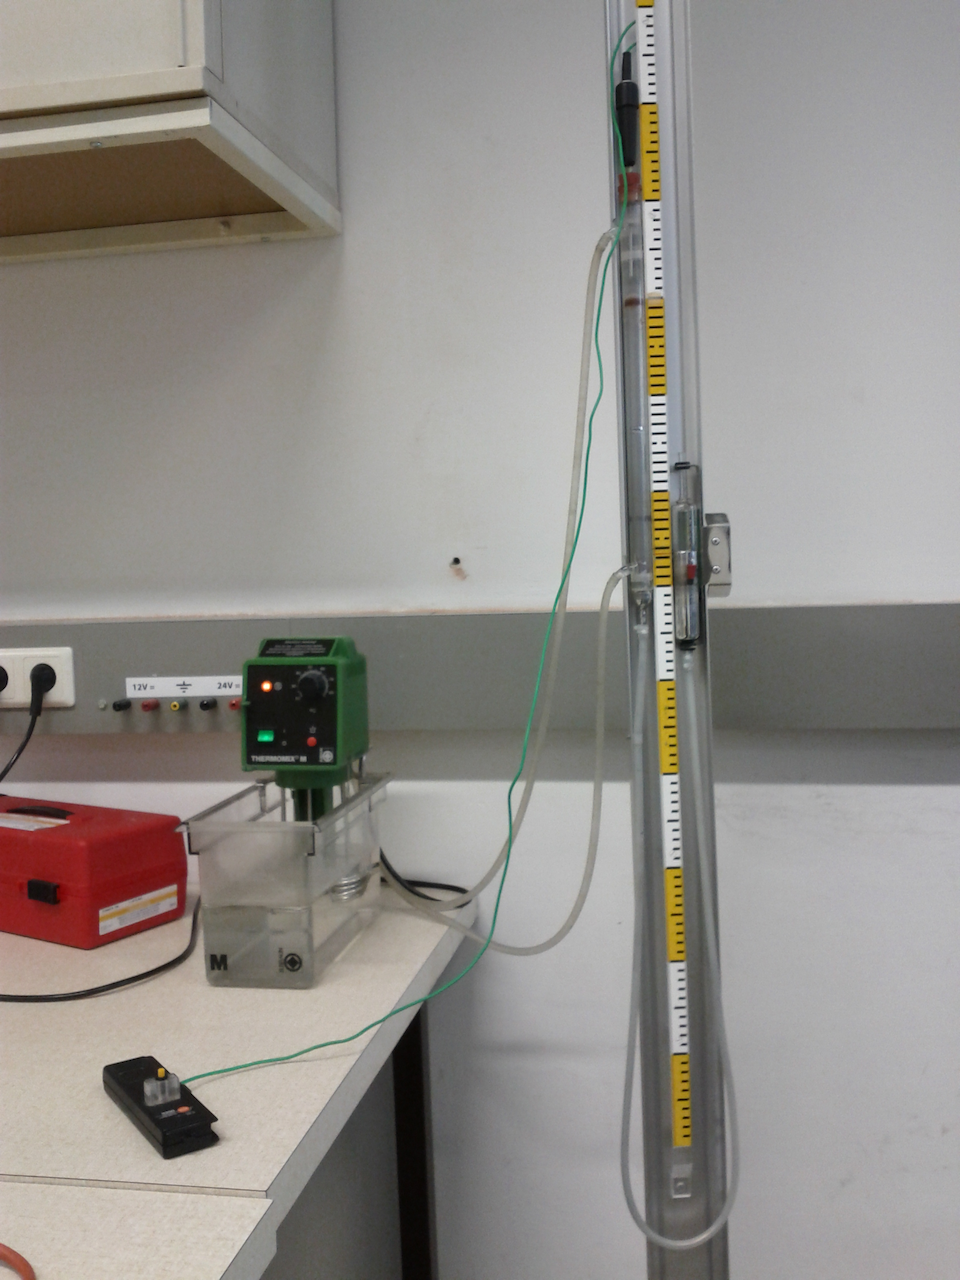
\includegraphics[scale=0.22]{./figure/gas_therm_aufbau.png}
	\caption{Versuchsaufbau mit Heizgerät und Thermometer}
	\label{fig:gas_therm_aufbau}
\end{figure}

%Equipment:
%\begin{itemize}
%	\item[-] Testoterm Sekundenthermometer (9200)
%	\item[-] Halterung mit Quecksilbergefüllten Röhren (siehe Abb. \ref{fig:gas_therm_aufbau} rechts)
%	\item[-] Heizgerät Thermomix B.Braun
%\end{itemize}

\subsection{Messwerte und Ergebnisse}
Luftdruck im Labor: $(993\pm 1)$mBar\\
Raumtemperatur: $(22 \pm 1)^\circ $C







%%%% TO DO SHORTY:
%%% bitte einheiten in die tabelle einfügen (2. zeile) und die spalte "Produkte" als Integerdarstellung statt der unpraktischen 10erpotenzen ausführen


\begin{figure}[H]
	\centering
	\pgfplotstabletypeset[
			columns={Druck, Laenge, Produkt, Fehler},
			%columns/Druck/.style={column name=$Druck\\[mmHg]$},
			col sep=&,
			every head row/.style={before row=\hline,after row=\hline\hline},
			every last row/.style={after row=\hline},
			every first column/.style={
								column type/.add={|}{}
							        },
			every last column/.style={
								column type/.add={}{|} 
								}
			]{
			Druck & Laenge & Produkt & Fehler
			%[mmHg] \pm1; [mm] \pm1; [mmHg*mm]; [mmHg*mm]
			917 &213 &195280 &950 
			794 &229 &181780 &830 
			745 &245 &182480 &790 
			713 &256 &182480 &760
			681 &266 &181090 &740 
	}
	\caption{Druck/Volumen bei Raumtemperatur}
	\label{fig:Messergebnis1_1}
\end{figure}


\end{multicols}

\begin{figure}[H]
	\centering
	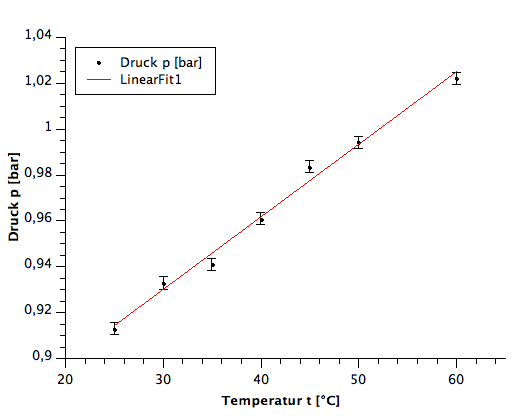
\includegraphics[scale=0.65]{./figure/Spannungskoeffizient-lin_Fit.png}
	\caption{Temperatur gegen mmHg-Differenz, linearer Fit}
	\label{fig:gas_therm_Spannungskoeffizient}
\end{figure}
%B (y-intercept) = 8,350436459016395e-01 +/- 3,812549620209208e-03
%A (slope) = 3,164236065573769e-03 +/- 9,031174786969129e-05

\begin{multicols}{2}



$$\frac{\Delta p}{\Delta \vartheta} = (3.164 \pm 0.091) mbar/ ^\circ C$$
$$ p_0 = (835.0 \pm 3.9) mbar$$\\
\\
$$\beta = (0.00379 \pm 0.00012) K^-1$$
$$T_0 =(263.9 \pm 8.0)K$$



\subsection{Diskussion}

Wie in Abbildung \ref{fig:Messergebnis1_1} zu sehen, liegen 4 der multiplizierten Druck/Länge Wertepaare, innerhalb der Unsicherheit, gut beieinander. Das Boyle-Mariott'sche Gesetz scheint also, in guter Näherung, auch für Luft zu gelten.\\
Einzig die erste Messung weicht deutlich ab. Mögliche Erklärungen dafür wären:\\
\indent - Ein Fehler beim Ablesen der Skala. Über die gesamte Arbeit am Gasthermometer wurden einige Messungen doppelt gecheckt und diskutiert, das die Kombination aus vielen nicht-durchnummerierten Strichen in der Vertikalen und der nicht-perfekten Sicht beider Durchführenden zu Unsicherheit geführt hat.\\
Da dieser Messwert aus der allerersten Kontrolle an der Skala überhaupt stammt, und dabei das Bewusstsein für dieses Problem noch nicht voll vorhanden war,  lässt sich ein Lesefehler hier nicht ausschließen.\\
\indent - Eine weitere Möglichkeit ist ein systematischer Fehler im Messaufbau, der erst bei größeren Abständen / Drücken anschlägt: Das erste Wertepaar wurde bei deutlich höherem Druck abgelesen, als alle anderen. Das bedeutet, dass sowohl der Höhenunterschied zwischen beiden Behältern verhältnismäßig groß ist, wie auch der Druck auf die Luft im Messgefäß. Möglicherweise ergeben sich bei extremeren Einstellungen ungewollte Effekte.\\
\\
Der ermittelte Spannungskoeffizient stimmt mit dem erwarteten Wert in Näherung überein. In Abbildung \ref{fig:gas_therm_Spannungskoeffizient} ist zu erkennen, dass die gemessenen Werte zwar sehr deutlich eine Gerade annähern, aber durchaus starke Schwankungen in beide Richtungen aufweisen.\\
Ein systematischer Fehler ist nicht zu erwarten. Die Schwankungen könnten der Messmethodik geschuldet sein, jedenfalls wären hier Verbesserungen sicher möglich:\\
Die Messkammer wird aufgeheizt und das Druckverhältnis für verschiedene Temperaturen gemessen. Aufgrund der begrenzten Zeit im Praktikum wurde versucht, das einigermaßen zügig durchzuführen. Da nicht nur die Luft sondern auch das Quecksilber im Messgerät erhitzt wird, entsteht eine Temperatur-Differenz zwischen dem Quecksilber im Messbehälter und demjenigen im Vorratsbehälter. Ein Halten des Systems auf gleichmäßiger Temperatur, für einige Minuten und vor jeder Messung, wäre möglicherweise besser.\\
Jedenfalls sind Fehler durch Material und Umgebung nicht auszuschließen, da innerhalb kurzer Zeit verschiedene Temperaturen durchgesteppt werden, jedoch nur in einem abgegrenzten Teil des Gasthermometers.\\
Schließlich sind auch etwaige Ablesefehler und -ungenauigkeiten, wie oben argumentiert, nicht auszuschließen.\\
Interessant wäre schließlich, wie gut das Ergebnis bei genauer linearen Messergebnissen wäre; Also wenn der Einfluss der Messung auf das Ergebnis sehr viel kleiner wäre und damit die Näherung, Luft (deren genaue Zusammensetzung uns hier auch unbekannt ist) als ideales Gas zu deuten, klarer erkennbar wäre.

\pagebreak

%%%%%%%%%%%%%%%%%%%%%%%%%%%%%%%%%%%%
\section{Adiabatenkoeffizient der Luft}
In diesem Experiment bestimmen wir den Adiabatenkoeffizienten der Luft. \\
Wird ein Gas komprimiert, ohne das Wärme entweichen kann, steigt der Druck stärker an als wenn die Wärme entweichen kann. Im Normalfall (isotherm) entspricht der Druck
$$p = \frac{C}{V}$$
wobei C eine Konstante ist.
Im adiabatischen Fall, den wir näherungsweise für Luft erhalten, welche ihren Druck in kurzen Intervallen ändert, entspricht dieser:
$$p = \frac{C}{V^\kappa}$$
Es gibt in der Theorie einen Zusammenhang zwischen dem Koeffizienten $\kappa$ und den Freiheitsgraden der Moleküle im Gas: Moleküle in Luft verfügen über 6 Freiheitsgrade (3 Raumdimensionen, 3 Rotationsachsen), wobei die Eigendrehung entlang der Achse quer durch das Molekül kaum einen bis keinen Beitrag leistet und daher vernachlässigt wird. Mit 5 Freiheitsgraden ergibt sich ein erwarteter Wert von
$$\kappa = \frac{f+2}{f} = \frac{7}{5} = 1.4$$
Um diesen Wert experimentell zu bestimmen verwenden wir ein 10L Gefäß und einen Gummi-Blasebalg, um eine Metallkugel in Schwingung zu versetzen. Die Periodendauer wird bestimmt, indem jeweils 5 ganze Schwingungen gemessen werden und so der Fehler für eine Periode klein gehalten wird.\\
Der Aufbau ist in \ref{fig:adiabatenkoeffizienten_aufbau} ersichtlich.
\begin{figure}[H]
	\centering
	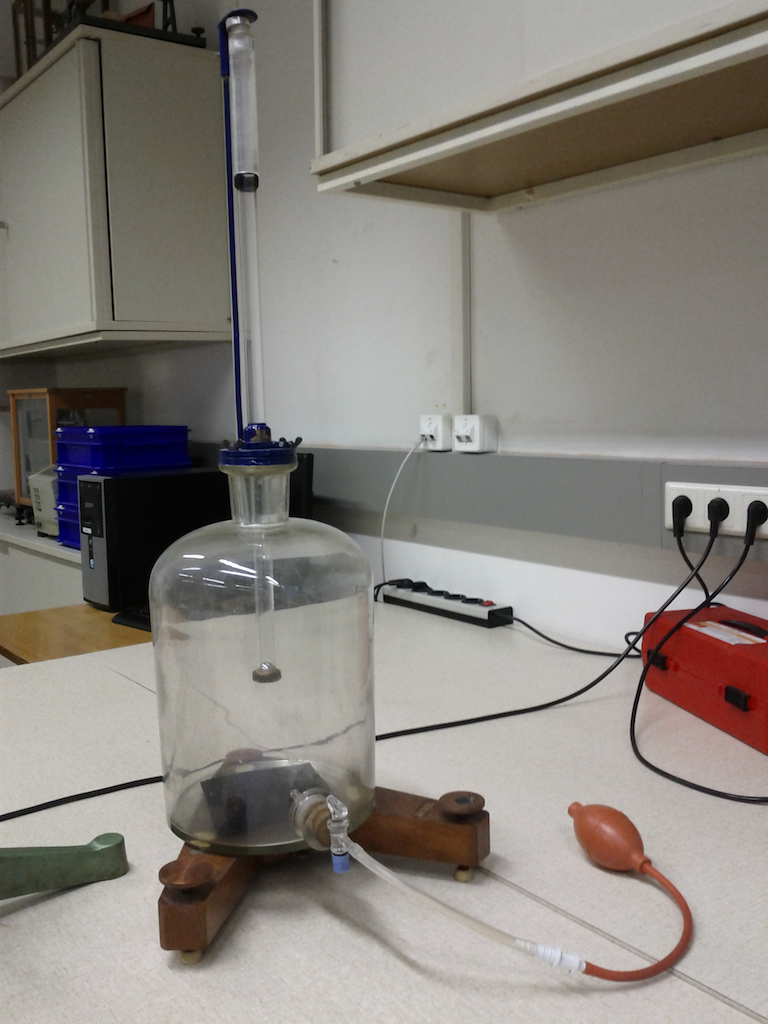
\includegraphics[scale=0.25]{./figure/koeffizient.png}
	\caption{Versuchsaufbau zur Ermittlung des Adiabatenkoeffizienten der Luft}
	\label{fig:adiabatenkoeffizienten_aufbau}
\end{figure}
\noindent
Nach der Herleitung (aus 3.1.3 [1]) erhalten wir folgende Formal für $\kappa$:
$$\kappa = \left(\frac{2\pi}{T}\right)^2  \frac{m V_0}{q^2  p}$$
T... Periodendauer der Schwingungen\\
m... Masse der Kugel\\
$V_0$... Volumen des Behälters\\
q... Querschnittsfläche der Röhre, in der sich die Kugel bewegt\\
p... Druck\\
\\
Der Druck lässt sich errechnen durch:
$$p = p_0 + \frac{m g}{q}$$
$p_0$... Außendruck (Luftdruck)\\
g... Erdbeschleunigung\\
\\
Aus den angegebenen Werten aus [1] 3.3.1, den gemessenen Zeiten für T, und der gemessenen Masse der Kugel errechnen wir im folgenden Abschnitt $\kappa$.
%Equipment:
%\begin{itemize}
%	\item[-] Stoppuhr
%	\item[-] Versuchsaufbau mit Pumpe und Metallkugel in Röhre
%\end{itemize}
%
\subsection{Messwerte und Ergebnisse}

Radius des Rohres: 8mm\\
Volumen des Gefäßes: 10l\\
Luftdruck p$_0$: 993 mbar\\
\\
Masse m der Kugel: $(16.828 \pm 0.008)g$ \\
\indent (Zwei Messungen:\\
Kugel mit Papier: $(18,638 \pm 0.005)g$\\
Schutzpapier allein: $(1,810 \pm 0.005)g$)\\

%Zwei Messungen, Kugel mit Papier, nur Papier => zwei mal Messfehler.\\
Werte von 3 mal 6 Messungen:
\begin{figure}[H]
	\centering
	\pgfplotstabletypeset[
			columns={T1,T2,T3},
			col sep=&,
			columns/T1/.style={column name=$T_1[s]$, precision=2, zerofill}, %\makecell{Line 1\\Line 2}
			columns/T2/.style={column name=$T_2[s]$, precision=2, zerofill},
			columns/T3/.style={column name=$T_3[s]$, precision=2, zerofill},
			every head row/.style={before row=\hline,after row=\hline\hline},
			every last row/.style={after row=\hline},
			every first column/.style={
								column type/.add={|}{}
							        },
			every last column/.style={
								column type/.add={}{|}
								}
			]{
			T1 & T2 & T3
			5.35 & 5.35 & 5.40
			5.49 & 5.36 & 5.37
			5.40 & 5.39 & 5.35
			5.37 & 5.49 & 5.41
			5.43 & 5.33 & 5.46
			5.31 & 5.46 & 5.44
			}
	\caption{Periodendauer nach 5 Schwingungen}
	\label{fig:adiabaten_periode_messung}
\end{figure}
\noindent
%Mean: 5,39778s $\approx$ 5.398s\\
%STABW: 0,05418s\\
%Standard Error of mean: 0.01277s $\approx$ 0.013s\\
($T_5 = (5.40 \pm 0.02)s$, siehe Abb. \ref{fig:adiabaten_periode_messung})
$$T=(1.08 \pm 0.01)s$$\\
\\
$$\kappa = ($$

\subsection{Diskussion}
Die Messungen gestalteten sich eher schwierig, da gut messbare Schwingungen nur mit etwas Aufwand zu bewerkstelligen sind. Dennoch ergab sich eine gute Messreihe wie in Tabelle \ref{fig:adiabaten_periode_messung} ersichtlich.
Da der Fehler bei der Messung der Kugelmasse von 0.005g zweimal in die Messung eingeht steigert der Fehler sich aufgerundet auf 0.008g. Unklar war das angegebene Volumen des in Abb. \ref{fig:adiabatenkoeffizienten_aufbau} zu sehenden Behälters. Mit 10L erschien das etwas überdimensioniert. Da unser Ergebnis mit $$\kappa = 1.32$$ sehr nahe am Wert liegt den man über die Freiheitsgrade erhält, scheint das Volumen doch zu zutreffen.

%%%%%% Dampfdichtebestimmung %%%%%%%%

\section{Dampfdichtebestim- mung}
In diesem Teil von PW5 wurde die Dampfdichte $\alpha$ von Aceton bestimmt.\\
Die Dampfdichte ist das Verhältnis der Dichte eines Gases zur Dichte von Luft. Da Aceton bei $0 ^\circ$C nicht gasförmig ist, sondern erst bei $56^\circ$C verdampft, wird Aceton näherungsweise als ideales Gas angenommen. So kann (nach der allgemeinen Gasgleichung) von Messungen bei höheren Temperaturen rückgerechnet werden. Durch Umformung kann daraus die Dichte des Gases durch andere bekannte/ gemessene Werte ausgedrückt werden.
$$\frac{p}{\rho_D \cdot T}= \frac{p_N}{\rho_N \cdot T_N}$$ 
(Gasgleichung dividiert durch die Masse)\\
Der Ausdruck für $\rho_N$ wird in $\alpha$ eingesetzt.
$$\alpha = \frac{\rho_N}{\rho_{L,N}}=\frac{\rho_D}{\rho_{L,N}} \cdot \frac{p_N T}{p \cdot T_N}$$
Da das Verhältnis der Dichten gleich dem der Molekularmassen ist, erhält man die Molekularmasse von Aceton, indem man $\alpha$ mit der von Luft multipliziert.\\
\\
Im Versuch wird Aceton in einem (auf $90^\circ$C erhitzten) Glaszylinder verdampft und verdrängt dabei Luft. Diese wird in einen mit Wasser gefüllten Messzylinder umgeleitet, in welchem das verdrängte Volumen abgelesen werden kann, und damit das Volumen des verdampften Acetons.
Da dieses rasch verdunstet, ist es wichtig, es schnell und und unmittelbar vor dem Verdampfen, zu wägen.\\
Außerdem sind noch Luftdruck, Höhe der Wassersäule und Raumtemperatur zu messen, sowie der Dampfdruck des gesättigten Wasserdampfes aus einer Tabelle zu entnehmen. Aus
$$\alpha = \frac{m}{V} \cdot \frac{760}{p} \cdot \frac{1 + \frac{1}{273.15} \cdot \vartheta}{0.001293}$$
wobei
$$p= Luftdruck - \frac{Wassersaeule}{13.6} - p_w$$
erhält man schließlich $\alpha$.

\subsection{Messwerte und Ergebnisse}

Raumtemperatur: $(23\pm 0.5)^\circ$C\\
Luftdruck: $(744.8 \pm 0.76)$ mmHg\\
Höhe der Wassersäule: $(688 \pm 2)$ mm\\
verdrängtes Volumen: $(57 \pm 0.2)$ cm$^3$\\
Masse$_{Aceton}: (0.177 \pm 0.08)$ g\\
\\
$$\alpha_{Aceton} = (2.95 \pm 0.14)$$
$$molare Masse = (85.2 \pm 4.1) g/mol$$



\subsection{Diskussion}
Die erwartete molare Masse von Aceton ist etwa $58.1$g/mol [2].\\
Das Ergebnis dieser Messung liegt zwar in der richtigen Größenordnung, ansonsten jedoch deutlich außerhalb der Unsicherheit.\\
Ein Nachfragen beim Betreuer und Mitstudierenden, die das Experiment bereits durchgeführt haben ergab, dass größere Abweichungen bei diesem Versuchsaufbau durchaus bekannt sind. Die Fehler der einzelnen Messgrößen wurden, auch deshalb, eher vorsichtig abgeschätzt. Dennoch ist der Unsicherheitsbereich klein gegenüber der Abweichung vom Literaturwert.\\
Diese Diskussion soll sich möglichen Ursachen, aber auch Grenzen der Machbarkeit, im Rahmen des Praktikums, widmen:\\
Der Aufbau des Versuches bietet einige Möglichkeiten, Fehler in die Messung zu bringen:\\
\indent - Es war unmöglich, die Wassersäule im Messzylinder sauber, ohne nennenswerte Luftblase zu installieren (ca. 2cm$^3$)\\
\indent - Um sicher zu gehen, dass nach Erhitzen des Kolbens keine Luft mehr entweicht, könnte man deutlich länger warten, als, wie hier, einige Minuten (< 5).
\indent - Das Kölbchen mit dem Aceton wird in den Verdampfungskolben fallen gelassen. Ob es hier, je nach Lage, nach dem Aufprall, zu Verzerrungen kommt, lässt sich ohne Weiteres nicht beantworten.\\
\\
\indent - Besonderes Augenmerk soll die Masse des Acetons erhalten: Es verdunstet schnell, und die verwendete Menge ist klein. Daher soll die Massenbestimmung unmittelbar und rasch vor der eigentlichen Messung erfolgen.\\
Sieht man die Masse in der Endgleichung als Parameter, stellt man fest, dass sich hier auch kleine Änderungen stark auf das Ergebnis auswirken (Veränderungen im 0.0x - Gramm Bereich ändern das Ergebnis um einige g/mol; Durch Veränderung der ersten Nachkommastelle der Masse in Gramm, lässt sich leicht das erwartete Ergebnis erreichen und sogar deutlich unterschreiten.\\
Die Vermutung liegt also nahe, dass vor allem hier ein deutlicher systematischer Fehler entsteht.\\
Eine sehr erste und einfache Möglichkeit, dieser Vermutung nachzugehen wäre, die Zeit zwischen dem Wägen und Einwerfen des Acetons in allen Gruppen bis zum Semesterende zu messen, und zu vergleichen, ob Schnelligkeit und Genauigkeit der Ergebnisse direkt proportional sind.\\
Eine technische Variante wäre, geschlossene Kapseln zum Wägen zu verwenden, die unmittelbar vor dem Verdampfen erst geöffnet werden.\\
Es wurde in dieser Gruppe bewusst rasch gewogen, einige Sekunden sind jedoch nicht zu vermeiden.\\
\\
Natürlich gibt es noch einige andere mögliche Ursachen des Ergebnisses (wie die Zusammensetzung des Acetons, Fehler in der Temperaturmessung, ungleichmäßige Temperatur uva.), jedoch liefert die außerordentlich hohe Auswirkung einer Änderung der Masse, auf das Ergebnis, einen starken Anhaltspunkt um hier weiterzusuchen, wäre das Experiment denn Teil einer größeren Forschung.


\section{Quellen}
[1] Leitfaden, \url{http://www.univie.ac.at/anfpra/neu1/pw/pw5/PW5_PL1.pdf}\\
[2] Lit-Wert Aceton, \url{http://de.wikipedia.org/wiki/Aceton}

\end{multicols}
\end{document}